% $Id: patches.tex 8981 2021-06-07 16:50:34Z mskala $

%
% MSK 008 patch suggestions
% Copyright (C) 2017  Matthew Skala
%
% This program is free software: you can redistribute it and/or modify
% it under the terms of the GNU General Public License as published by
% the Free Software Foundation, version 3.
%
% This program is distributed in the hope that it will be useful,
% but WITHOUT ANY WARRANTY; without even the implied warranty of
% MERCHANTABILITY or FITNESS FOR A PARTICULAR PURPOSE.  See the
% GNU General Public License for more details.
%
% You should have received a copy of the GNU General Public License
% along with this program.  If not, see <http://www.gnu.org/licenses/>.
%
% Matthew Skala
% https://northcoastsynthesis.com/
% mskala@northcoastsynthesis.com
%

\chapter{Patch Suggestions}

The MSK~008 provides simple building blocks that can be combined and applied
in a number of ways, some of which are hard to describe or very much
specific to individual larger patches.  It's what is sometimes called a
``patch-programmable'' module.  The suggestions in this chapter are
intended to inspire readers to devise their own and \emph{not} to be a
complete list of every possible way to use the module.

\section{Basic octave switch and transposition}

Basic use as a manually-controlled octave switch:  pitch CV into the CV1
input, output into oscillator, switch the toggle switch up or down to go up
or down an octave.  Either channel can be patched like this and the other
remains available for some other use; with no other inputs patched, the
second channel can (through normalization) drive a second oscillator with
independent manual octave switching.

In this patch it's also possible to do a CV-controlled transposition by
feeding the transposition voltage into the CV2 input.  On the left, it
transposes in the same direction as the input; on the right, it is inverted;
and the same transposition voltage can be used for both at once through the
normalization.

{\hspace*{\fill}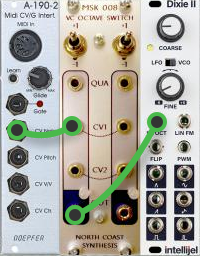
\includegraphics[scale=0.8]{patch1.png}\hspace*{\fill}\par} 

\section{CV-controlled octave switch}

The QUA input (here driven by an attenuated sine wave LFO) has a similar
effect to switching the manual switch, but can go from $-$2 to $+$2 octaves.

{\hspace*{\fill}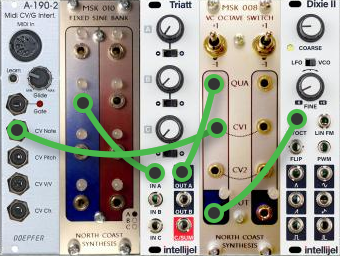
\includegraphics[scale=0.8]{patch2.png}\hspace*{\fill}\par} 

\section{Switching by other musical intervals}

An oscillator or other module with an ``exponential FM'' input can switch up
or down by some other interval, such as a perfect fifth, by adjusting the
attenuation on the exponential FM.  Here the MSK~008 is functioning as
a manually controlled $\pm$1V offset generator; as before, patching an LFO
into the QUA input would allow the same thing under CV control.

{\hspace*{\fill}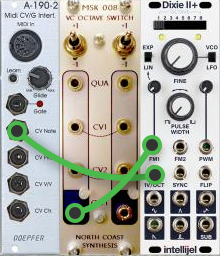
\includegraphics[scale=0.8]{patch8.png}\hspace*{\fill}\par} 

\section{Wavefolding}

Basic wavefolder patch.  The input signal is mult-ed to both the QUA input
and CV2 on the inverting channel.  To understand its operation, imagine the
rising slope of a sawtooth wave on the input.  The quantizer changes that
into a stair-step, and then the subtraction changes each step of the stair
into a little falling sawtooth slope.  The picture shows the input going
through a VCA, which could be used as a manual attenuator or under CV
control to modulate the amount of folding effect; a little slow modulation
makes the sound much more animated and interesting.  Output voltage for this
patch is low (1V peak to peak, unless the input is hot enough to exceed the
quantization range) and it may need amplification in some applications.  For
a stronger output (up to 4V peak to peak), try feeding the input only into
the QUA input (not also CV2), which gives a slightly less aggressive
bit-crushing sound and works in either channel.

{\hspace*{\fill}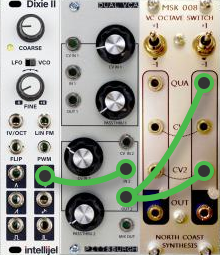
\includegraphics[scale=0.8]{patch3.png}\hspace*{\fill}\par} 

\section{Scale degree detector}

This is an extended application of the wavefolder patch, originating in a
discussion on a Web forum about how to detect a given scale degree for
switching sequencer patterns in a self-generating melody.  It's to be
understood that the details would vary a lot depending on the exact
application, but this example illustrates some useful tricks for getting the
most out of the module.

\noindent
{\hspace*{\fill}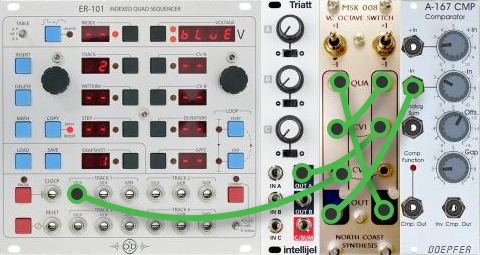
\includegraphics[scale=0.5]{patch4.png}\hspace*{\fill}\par} 

The sequencer generates a pitch control voltage, here assumed to be from 0V
to 5V (an actual ER-101 is capable of a wider range, but I'm only using it
as a recognizable example of a sequencer, not meaning to imply that the
input would necessarily really be an ER-101 in practice).  That voltage goes
into the CV2 input of \emph{both} channels through the normalization.  So in
the right channel, we are subtracting the pitch voltage from an offset
generated by the Triatt, which will be nominally $+$2.5V.  Ignore the QUA
input of the right channel for the moment.  The output on the right ranges
from $+$2.5V down to $-$2.5V as the pitch CV \emph{increases}, and that goes
into the QUA input of the left channel.

The left channel's quantizer recognizes which octave we are in, with a
quantizer output of $+$2V for the first octave (pitch CV from 0V to 1V,
right channel output from $+$2.5V down to $+$1.5V), $+$1V for the second
octave, and so on.  To the quantizer output we add the original pitch CV. 
So as long as the pitch CV remains in the range 0V to 5V, the output of the
left channel is in the range 2V to 3V, expressing what can be called the
``pitch class,'' pitch modulo octave, or scale degree within the octave. 
For example, if C in one octave is 0V on the input, then C in any octave
will be 2V on the output, and F$\sharp$ in any octave will be 2.5V on the
output.  This output then goes into other modules, here depicted by an A-167
comparator, to detect when the sequencer hits a given scale degree.  That
might be used to trigger a change in the sequencer pattern or something.

In order to have the output range be 2V to 3V and not the less convenient
4.5V to 5.5V, we need to defeat the normalization on the left channel CV1
input.  It would work to just plug in a patch cable there with nothing on
the other end, but people don't like having loose cable ends floating
around, so the diagram shows this input patched into the right channel's QUA
input, which (with the offset switch in the centre 0 position) has a very
high impedance and is effectively the same as leaving the cable unpatched,
but looks tidier.  The CV1 input itself is 100k$\Omega$ into a
virtual ground and will not have any unexpected effects on the right
channel.  For other output ranges instead of 2V to 3V, one could apply an
appropriate positive or negative offset to the left channel CV1 input
instead.

The exact cut-off point for the octaves can be adjusted by adjusting the
offset into the right-channel CV1.  In the simplest case one could just mult
the pitch CV into QUA and CV2 of the right channel in the basic wavefolder
patch, leaving the left channel free for other purposes; but that would give
a $\pm$2.5V input range, $\pm$0.5V output range, inversion of the voltages,
and no control over the cut-off point; so it might not be useful in as many
patches.

\section{Mid-side and fake stereo}

With signals fed into the CV1 and CV2 inputs, normalled across to both
channels, the two outputs of the MSK~008 are the sum and difference of the
two signals.  As a result it functions as a ``mid-side'' encoder or decoder,
with 6dB of gain across the pair if you use two of them with nothing in
between.  In this example we've got a mono signal going into a Doepfer
A-188-1 bucket brigade delay.  The dry signal (through the mult built into
the Doepfer module) goes into CV1 on the MSK~008 to be the ``mid'' signal
applied to both stereo channels.  The BBD's mix knob is set to fully wet
output, and that goes into CV2 to be the ``side'' signal for mid-side
decoding, applied with opposite phase to the right and left.

The result is a fast echo and phase cancellation on the two stereo channels;
a ``fake stereo'' effect that spreads mono material across the sound stage
as if it had been recorded in stereo.  It's not very realistic, but a
similar effect was historically important.  When stereo recording was new,
Capital Records sold a lot of vinyl that they called ``Duophonic,'' with
essentially this effect applied to mono masters in order to appeal to people
with new stereo hi-fi equipment.

Other interesting effects can be had by using filters, distortion, and other
things instead of or in addition to the BBD.

{\hspace*{\fill}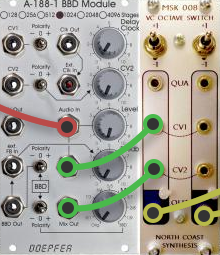
\includegraphics[scale=0.8]{patch5.png}\hspace*{\fill}\par} 

\section{Basic Schmitt trigger patch}

With the output fed back into the QUA input, either channel can function as
a Schmitt trigger: that is, a comparator with hysteresis.  When the sum of
the other inputs (taking into account any inversion) is greater than $+$2.5,
the module switches into the positive state (quantizer output $+$2V).  When
the sum is less than $-$2.5V, the module switches into the negative state
(quantizer output $-$2.5V).  In between, it retains its current state.  This
behaviour can be used for a number of switching and distortion effects,
detecting peaks, and so on.  However, in the simplest single-channel
version, it is not particularly well-behaved; in particular, the input
voltages appear superimposed on the output, and the basic states are
$\pm$2V, which may not be what other logic modules expect.

{\hspace*{\fill}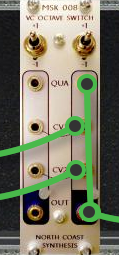
\includegraphics[scale=0.8]{patch7.png}\hspace*{\fill}\par} 

\section{Gate stretcher/delay}

Here's an application of the Schmitt trigger patch.  An ADSR envelope
generates a voltage input for the Schmitt trigger.  The toggle switch for
that channel is set to $-$1 to ensure that when the ADSR is at 0V, the
module output will be biased into the negative state.  When the ADSR
receives a gate signal, its output voltage starts to increase; eventually it
rises enough to trip the MSK~008 into the positive state, and the delay
before that happens is controlled by adjusting the attack time.  Similarly,
when the gate disappears, the ADSR generator goes into its release phase,
and there is a delay controlled by release time before it will switch the
MSK~008 into the negative state.

The Doepfer A-140 is shown as an example of a typical envelope generator,
but one could also use any common ``AD''-style envelope generator, and if it
is desired to use this patch for stretching a trigger signal (which is
nothing but a very short gate) into something longer, with a delay longer
than the trigger duration, then it might be important to choose an envelope
generator that will go through its full attack cycle despite having a very
short trigger input.

{\hspace*{\fill}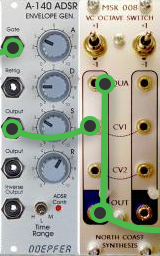
\includegraphics[scale=0.8]{patch6.png}\hspace*{\fill}\par} 

The deluxe version of the patch uses the second channel of the MSK~008, and
an offset input (typically 2V), to clean up the output voltage a bit. 
Minor stair-stepping is still possible.

{\hspace*{\fill}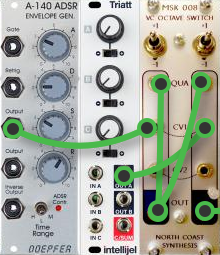
\includegraphics[scale=0.8]{patch9.png}\hspace*{\fill}\par} 
